\section{Mạng Nơ-ron}
    % \subsubsection{Đơn vị Nơ-ron cơ bản}
    % Tương tự như thuật toán tiến hóa, mạng Nơ-ron hay còn gọi là mạng Nơ-ron nhân tạo cũng là một ý tưởng được lấy cảm hứng từ mạng Nơ-ron thần kinh của con người. Trong đó, Nơ-ron thần kinh là một đơn vị cơ bản cấu tạo hệ thống thần kinh quan trọng nhất của bộ não, nó có cấu trúc được mô tả như hình bên dưới:
    % \begin{figure}[ht]
    %     \centering
    %     \fbox{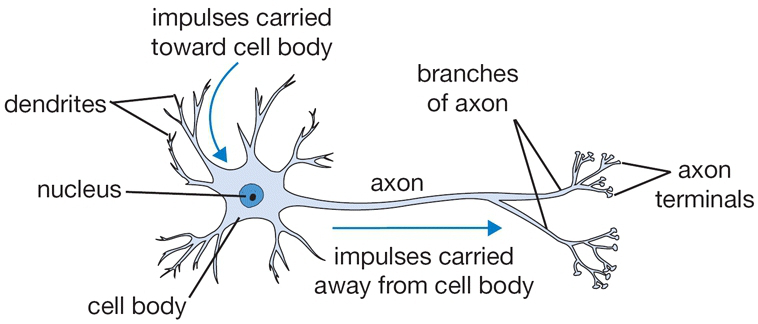
\includegraphics[width=\linewidth]{neuron-human.png}}
    %     \caption{Cấu trúc của một Nơ-ron đơn lẻ hay còn gọi là perceptron}
    %     \label{fig:problem:human-neuron}
    % \end{figure}
    % Một đơn vị Nơ-ron đơn lẻ được gọi là \emph{perceptron}. Từ mô hình của \emph{perceptron} được mô tả trong hình \ref{fig:problem:human-neuron} có thể thấy mỗi một Nơ-ron sẽ nhận nhiều đầu vào nhưng chỉ cho ra một kết quả duy nhất. Được biểu diễn dưới dạng mô hình như sau:
    % \begin{figure}[ht]
    %     \centering
    %     \fbox{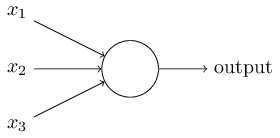
\includegraphics[width=0.7\linewidth]{perceptron.png}}
    %     \caption{Cấu trúc của một perceptron nhân tạo}
    %     \label{fig:problem:perceptron}
    % \end{figure}
    % Một \emph{perceptron} sẽ nhận một hoặc nhiều đầu $x$ vào dạng nhị phân và cho ra một kết quả $o$ dạng nhị phân duy nhất. Các đầu vào được điều phối tầm ảnh hưởng bởi các tham số trọng lượng tương ứng $w$ của nó, còn kết quả đầu ra được quyết định dựa vào một ngưỡng quyết định $b$ nào đó.
    \subsubsection{Kiến trúc mạng Nơ-ron}
    Mạng Nơ-ron là kết hợp của các tầng \emph{perceptron} hay còn gọi là \emph{perceptron} đa tầng. 
    \begin{figure}[ht]
        \centering
        \fbox{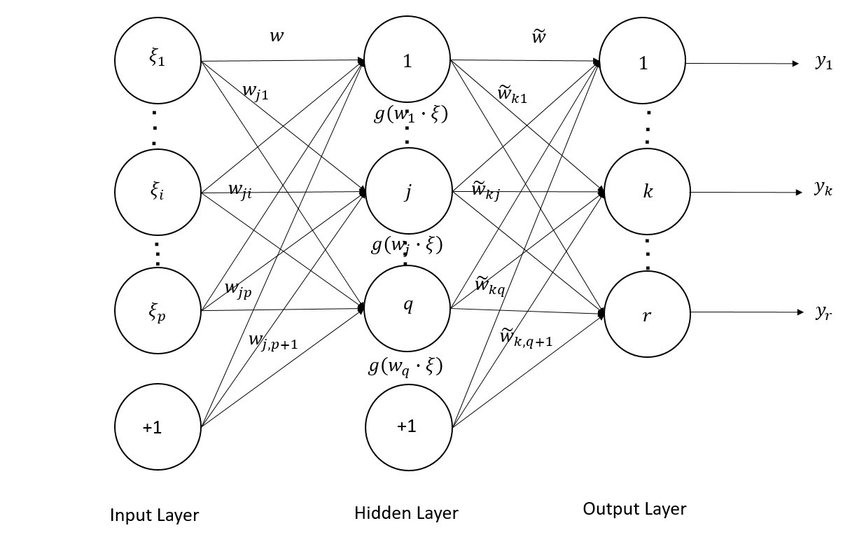
\includegraphics[width=\linewidth]{ff-neural.png}}
        \caption{Kiến trúc mạng Nơ-ron}
        \label{fig:problem:neural-architect}
    \end{figure}
    Một kiến trúc mạng Nơ-ron bao gồm 3 kiểu tầng chính:
    \begin{enumerate}
        \item \textbf{Tầng vào} (input layer): Là tầng bên trái cùng của mạng thể hiện cho đầu vào của mạng.
        \item \textbf{Tầng ẩn} (hidden layer): Là tầng nằm giữa tầng vào và tầng ra của mạng thể hiện cho các suy luận logic của mạng.
        \item \textbf{Tầng ra} (output layer): Là tầng nằm bên phải cùng của mạng thể hiện cho các đầu ra của mạng. Một mạng có thể có một hoặc nhiều đầu ra.
    \end{enumerate}
    Ở mỗi tầng, số lượng các nút mạng (nơ-ron) có thể khác nhau tuỳ thuộc vào bài toán và cách giải quyết. Nhưng thường khi làm việc các tầng ẩn thường có số lượng nơ-ron bằng nhau. 
    \subsubsection{Mạng Nơ-ron lan truyền tiến}
    Như hình \ref{fig:problem:neural-architect} có thể thấy tất các nút mạng được kết hợp đôi một với nhau theo một chiều duy nhất từ tầng vào đến tầng ra. Tức là mỗi nốt ở tầng nào đó sẽ nhận đầu vào từ các nốt ở tầng trước đó mà không có chiều suy luận ngước lại. Hay nói cách khác mạng Nơ-ron là này là một mạng Nơ-ron lan truyền tiến. 
    \begin{equation}
      \begin{array}{l}
        z_i^{l+1} = \sum_{j=1}^{n^{(l)}}w_{ij}^{(l+1)}a_j^{(l)} + b_j^{(l+1)} \\
        \\
        a_i^{(l+1)} = g(z_i^{(l+1)})
      \end{array}
    \end{equation}
    Trong đó $n^{(l)}$ là số lượng nút ở tầng $l$ tương ứng và $a_j^{(l)}$ là nút mạng thứ $j$ của tầng $l$. Còn $w_{ij}^{(l+1)}$ là tham số trọng lượng đầu vào $a_j^{(l)}$ đối với nút mạng thứ $i$ của tầng $l+1$ và $b_j^{(l+1)}$ là độ lệch thiên kiến ($bias$) của nút mạng thứ $i$ tầng thứ $l+1$. Đầu ra của nút mạng này được biểu diễn bằng $a_i^{(l+1)}$ ứng với hàm kích hoạt $g(z_i)$ tương ứng. Và riêng với tầng vào (input layer), thông thường $a^{(1}$ cũng chính là các đầu vào $x$ tương ứng của mạng. 
    \subsubsection{Huấn luyện mạng Nơ-ron}
    Trước khi giải thích làm thế nào để huấn luyện mạng Nơ-ron thì ta sẽ cần định nghĩa về \emph{hàm lỗi} (loss function). Hàm lỗi là hàm cho ta biết mạng nơ-ron hiện tại đang tốt như thế nào trên một tác vụ, bộ dữ liệu cụ thể. Một cách tiếp cận trực quan và đơn giản nhất mà ta có thể nghĩ ra đó là sử dụng hàm trung bình bình phương lỗi (Min Square Error - MSE).
    \begin{equation}
      L(y, \widehat{y}) = \frac{1}{m}\sum_{i=1}^m(y_i - \widehat{y_i})^2
    \end{equation}
    Với $\widehat{y}$ là giá trị ước lượng từ mạng, $y$ là giá trị thực tế từ bộ dữ liệu huấn luyện. Nếu giá trị hàm lỗi lớn chứng tỏ mô hình mạng nơ-ron của ta chênh lệch nhiều, chưa đưa ra kết quả tốt. Nhiệm vụ của ta sẽ là tối ưu bộ tham số $(w,b)$ sao cho hàm lỗi nhỏ nhất có thể. Và đây cũng là ý tưởng chính trong việc \textbf{huấn luyện} mạng nơ-ron. Để thực hiện nhiệm vụ tối ưu này, có 2 lớp phương pháp chính:
    \begin{itemize}
        \item Lớp thuật toán sử dụng phương pháp \textbf{gradient-based}.
        \item Lớp thuật toán \textbf{tiến hóa - EA}.
    \end{itemize}
    Hầu hết các nhóm nghiên cứu đều sử dụng phương pháp gradient-based để huấn luyện mạng nơ-ron hơn là sử dụng các phương pháp tiến hóa. Tuy nhiên cho đến nay các phương pháp gradient-based bắt đầu bộc lộ nhiều hạn chế, vì nó chỉ tạo ra được công cụ để giải quyết bài toàn ban đầu mà con người đưa thông số cho lời giải, bộ dữ liệu mẫu. Một số bài toán phức tạp mà việc xác định đầu ra thực tế (cặp input-output) là không thể hoặc gặp nhiều cản trở như tối ưu \emph{policy} trong mô hình học tăng cường, hay bài toán \emph{AutoML}. Trong khi trí thông minh của sinh vật có từ sự chủ động, là kết quả của quá trình tiến hóa nên một số nhóm nghiên cứu nổi tiếng như Google Brain, OpenAI, Uber đã đưa ra một số kết quả trong việc áp dụng giải thuật tiến hóa trong việc huấn luyện mạng nơ-ron để giải quyết bài toán của mình.
    Bởi vậy trong đồ án này tôi sẽ trình bày về phương pháp thứ 2 sử dụng ý tưởng tiến hóa để huấn luyện mạng Nơ-ron. Mà cụ thể là áp dụng giải thuật tiến hóa đa nhiệm 2 - MFEAII để huấn luyện nhiều mạng Nơ-ron đồng thời.
\section{Tiến hóa đa nhiệm trong mạng Nơ-ron}
    Phương pháp sử dụng thuật toán tiến hóa để huấn luyện mạng nơ-ron hay còn gọi là \textbf{neuroevolution} xem vấn đề cần học giống như một bài toán tối ưu hộp đen (black-box optimisation) nơi các giải pháp được cải thiện qua các thế hệ tiến hóa. Neuroevolution sử dụng thuật toán tiến hóa để xây dựng, huấn luyện mạng nơ-ron bao gồm các tham số, cấu trúc của mạng. Trong Neuroevolution, một mẫu gen (gennotype) là kiểu cá thể của quần thể sẽ được ánh xạ với các tham số trong mạng Nơ-ron. Qua mỗi thế hệ tiến hóa các cá thể sẽ được đánh giá dựa theo hàm đánh giá tương ứng với bài toán để chọn lọc và tiếp tục xây dựng thế hệ tiếp theo.
    
    
    Tuy nhiên một vấn đề nảy sinh trong việc huấn luyện mạng nơ-ron đó là việc không khai thác được những tri thức đã học được trong các mô hình đã học được trước đó. Chẳng hạn với bài toán nhận diện khuôn mặt, cho trước một mô hình đã được huấn luyện dựa theo bộ dữ liệu đã được xử lý dựa theo các đặc tính của khuôn mặt. Trong tương lai khi muốn thêm các đặc tính khác vào bộ dữ liệu hoặc thay đổi cấu trúc của mạng thì việc phải huấn luyện lại từ đầu mà không tận dụng được mô hình trước đó là điều không thể tránh khỏi. Bằng ý tưởng của thuật toán tiến hóa đa nhiệm đã được trình bày ở phần trên thì việc áp dụng tiến hóa đa nhiệm vào huấn luyện mạng nơ-ron có thể giải quyết được vấn đề này. Tiến hóa đa nhiệm sẽ khai phá được mối quan hệ tiềm ẩn giữa các tác vụ có liên quan đến nhau, qua đó đẩy nhanh tốc độ hội tụ của các tác vụ.
    
    Tuy nhiên cần phải lưu ý rằng chữ \textbf{tác vụ} khi áp dụng tiến hóa đa nhiệm vào huấn luyện mạng nơ-ron có thể hiểu theo nhiều nghĩa.
    \begin{itemize}
        \item Cách hiểu thứ nhất: Mỗi tác vụ là một bộ dữ liệu có số lượng hoặc tính chất của thuộc tính khác nhau. Như ví dụ về bài toán nhận diện khuôn mặt, mỗi tác vụ tương ứng với bộ dữ liệu gồm số lượng thuộc tính khác nhau hoặc số lượng giống nhau nhưng lại thuộc các quốc gia khác nhau. 
        \item Cách hiểu thứ hai: Mỗi tác vụ tương ứng với một cấu trúc mạng khác nhau, có thể được biểu diễn dưới dạng mô-đun. 
    \end{itemize}
    Với mỗi cách hiểu sẽ tương ứng với một lớp bài toán khác nhau cần xây dựng mô hình riêng để giải quyết. Trong đồ án này tôi sẽ đưa ra các đề xuất của mình để giải quyết lần lượt cả 2 lớp bài toán trên.
    \begin{itemize}
        \item Với lớp bài toán thứ nhất tôi sẽ trình bày ở chương \ref{chap:problem_rl} trong việc áp dụng tiến hóa đa nhiệm trong việc huấn luyện mô hình học tăng cường trên nhiều môi trường đồng thời.
        \item Với lớp bài toán thứ hai tôi sẽ trình bày tại chương \ref{chap:problem} trong việc áp dụng tiến hóa đa nhiệm huấn luyện nhiều mạng nơ-ron với cấu trúc mô-đun.
    \end{itemize}
    Lưu ý rằng \emph{tiến hóa đa nhiệm} mà tôi nhắc tới sẽ là việc áp dụng đồng thời cả MFEA và MFEAII. Trong đó MFEA-II sẽ là thuật toán chủ yếu tôi muốn trình bày và MFEA sẽ là thuật toán cơ sở để so sánh, bên cạnh thuật toán tiến hóa thông thường (EA).
    

